\documentclass[master=cws,masteroption=ai]{kulemt}
\setup{title={Describing Images with Natural Language},
  author={Thijs Dieltjens \\ Wout Vekemans},
  promotor={Prof.\,dr.\,ir.\ Marie-Francine Moens},
  assessor={Ir.\,W. Eetveel},
  acyear={2015 -- 2016},
  assistant={Ir.\ S. Zoghbi}}
% De volgende \setup mag verwijderd worden als geen fiche gewenst is.
\setup{filingcard,
  translatedtitle={The best master thesis ever},
  udc=621.3,
  shortabstract={Hier komt een heel bondig abstract van hooguit 500
    woorden. \LaTeX\ commando's mogen hier gebruikt worden. Blanco lijnen
    (of het commando \texttt{\string\pa r}) zijn wel niet toegelaten!
    \endgraf \lipsum[2]}}
% Verwijder de "%" op de volgende lijn als je de kaft wil afdrukken
% \setup{coverpageonly}
% Verwijder de "%" op de volgende lijn als je enkel de eerste pagina's wil
% afdrukken en de rest bv. via Word aanmaken.
%\setup{frontpagesonly}

% Kies de fonts voor de gewone tekst, bv. Latin Modern
\setup{font=lm}

% Hier kun je dan nog andere pakketten laden of eigen definities voorzien

\usepackage{url}
\usepackage{todonotes}
% Tenslotte wordt hyperref gebruikt voor pdf bestanden.
% Dit mag verwijderd worden voor de af te drukken versie.
% \usepackage[pdfusetitle,colorlinks,plainpages=false]{hyperref}

%%%%%%%
% Om wat tekst te genereren wordt hier het lipsum pakket gebruikt.
% Bij een echte masterproef heb je dit natuurlijk nooit nodig!
\IfFileExists{lipsum.sty}%
 {\usepackage{lipsum}\setlipsumdefault{11-13}}%
 {\newcommand{\lipsum}[1][11-13]{\par Hier komt wat tekst: lipsum ##1.\par}}
%%%%%%%

%\includeonly{hfdst-n}
\begin{document}

\begin{preface}
  Dit is mijn dankwoord om iedereen te danken die mij bezig gehouden heeft.
  Hierbij dank ik mijn promotor, mijn begeleider en de voltallige jury.
  Ook mijn familie heeft mij erg gesteund natuurlijk.
\end{preface}

\tableofcontents*

\begin{abstract}
  In dit \texttt{abstract} environment wordt een al dan niet uitgebreide
  samenvatting van het werk gegeven. De bedoeling is wel dat dit tot
  1~bladzijde beperkt blijft.

  \lipsum[1]
\end{abstract}

% Een lijst van figuren en tabellen is optioneel
%\listoffigures
%\listoftables
% Bij een beperkt aantal figuren en tabellen gebruik je liever het volgende:
\listoffiguresandtables
% De lijst van symbolen is eveneens optioneel.
% Deze lijst moet wel manueel aangemaakt worden, bv. als volgt:
\chapter{Lijst van afkortingen en symbolen}
\section*{Afkortingen}
\begin{flushleft}
  \renewcommand{\arraystretch}{1.1}
  \begin{tabularx}{\textwidth}{@{}p{12mm}X@{}}
    LoG   & Laplacian-of-Gaussian \\
    MSE   & Mean Square error \\
    PSNR  & Peak Signal-to-Noise ratio \\
  \end{tabularx}
\end{flushleft}
\section*{Symbolen}
\begin{flushleft}
  \renewcommand{\arraystretch}{1.1}
  \begin{tabularx}{\textwidth}{@{}p{12mm}X@{}}
    42    & ``The Answer to the Ultimate Question of Life, the Universe,
            and Everything'' volgens de \cite{h2g2} \\
    $c$   & Lichtsnelheid \\
    $E$   & Energie \\
    $m$   & Massa \\
    $\pi$ & Het getal pi \\
  \end{tabularx}
\end{flushleft}

% Nu begint de eigenlijke tekst
\mainmatter

\chapter{Inleiding}
\label{inleiding}
In dit hoofdstuk wordt het werk ingeleid. Het doel wordt gedefinieerd en er
wordt uitgelegd wat de te volgen weg is (beter bekend als de rode draad).

Als je niet goed weet wat een masterproef is, kan je altijd
Wikipedia\cite{wiki} eens nakijken.

\section{Lorem ipsum 4--5}
\lipsum[4-5]

\section{Lorem ipsum 6--7}
\lipsum[6-7]

%%% Local Variables: 
%%% mode: latex
%%% TeX-master: "masterproef"
%%% End: 

\chapter{Gerelateerd werk}
\label{hoofdstuk:related}
Het automatisch genereren van beschrijvingen voor ongeziene afbeeldingen is een complex proces. Het combineert namelijk zowel computervisie (CV) als natuurlijke taalverwerking (NLP). Vele modellen zijn al voorgesteld die telkens elementen uit beide onderzoeksvelden combineren. 

Dit hoofdstuk begint met een vergelijking van verschillende mogelijkheden om afbeeldingen en zinnen voor te stellen. De meest relevante onderzoeken uit CV en NLP komen aan bod. Daarna volgt een samenvatting van de verschillende mogelijkheden om deze technologie\"en te integreren in \'e\'en model. 

Doorheen de jaren is deze integratie op verschillende manieren aangepakt. Het probleem van automatische afbeeldingsbeschrijving werd eerst niet beschouwd als generatieprobleem maar als opvraag- of \emph{retrievalprobleem}. Hierbij zoekt een model naar de beste zin in een bestaande verzameling van zinnen op basis van de ingevoerde foto \cite{Hodosh2013}. Nieuwere papers behandelen het probleem als een vertaalprobleem naar analogie met automatisch vertalen. Hierbij gebruikt men een codeer-decodeersysteem waarbij de afbeelding als brontaal wordt beschouwd en het Engels als doeltaal. Dit hoofdstuk biedt een overzicht van deze recentste technieken.

\section{Representatie van afbeeldingen}
Alle recente modellen gebruiken technieken uit computervisie om nuttige kenmerken af te leiden uit afbeeldingen. Kenmerken bevatten onder andere gedetecteerde acties, sc\`enes en objecten met hun attributen en relaties\cite{Bernardi}. Deze kenmerken vormen de basis voor een representatie van de afbeelding die als input dient voor het generatie- of opvraagmodel.

Eerst volgt een bespreking van technieken uit het verleden. Daarna beschrijft deze sectie Convolutionele Neurale Netwerken (CNN), die in de meer recente literatuur veelvuldig voorkomen.


\subsection{Oorspronkelijke CV modellen}
De literatuur gebruikt meerdere technieken uit computervisie om nuttige features of kenmerken af te leiden uit afbeeldingen. Kenmerken die in de vroegste papers over dit onderwerp voorkomen zijn bijvoorbeeld het type van de algemene sc\`ene, gedetecteerde objecten en attributen van deze objecten\cite{Farhadi2010,Patterson2014,Yang2011}.

Bij sc\`eneclassificatie leert een model voor ongeziene afbeeldingen een bepaalde algemene sc\`ene (bijvoorbeeld restaurant, slaapkamer, keuken) af te leiden. Ook modellen die verschillende objecten detecteren hebben hun nut. Van zulke gevonden objecten kunnen classifiers ook nog nuttige attributen zoals kleur bepalen. Om zulke afleidingen te maken, gebruiken de papers bestaande classifiers en detectoren zoals bij Felzenswalb et al.\cite{Felzenszwalb2008}, Im2Text\cite{Ordonez2011} en GIST\cite{Oliva2006}. Ee\'n of meerdere van deze features kan dan rechtstreeks de representatie vormen van een afbeelding. Daarnaast vormen deze features in een aantal werken\cite{Farhadi2010,Li2011,Mitchell2012,Yang2011} enkel de input voor abstracte afbeeldingsrepresentaties in de vorm van tupels. Deze tupels bevatten dan objecten, acties tussen objecten, sc\`enetypes en/of ruimtelijke relaties.

Een andere manier om afbeeldingen voor te stellen is het gebruik van Visual Dependency Representations (VDR) zoals voorgesteld door Elliott et al.\cite{Elliott2013}. Dit model werkt analoog aan een taalgebaseerde afhankelijkheidsgrammatica. Dit type grammatica stelt de syntactische structuur van een zin voor met woorden met daartussen binaire semantische of syntactische relaties\cite{Jurafsky:2009:SLP:1214993}. Figuur \ref{fig:dep_grammar} toont een voorbeeld van een zin ontleed met een afhankelijkheidsgrammatica. De gelabelde pijlen stellen de verschillende relaties tussen de woorden voor.

\begin{figure}[tb]
      \centering
      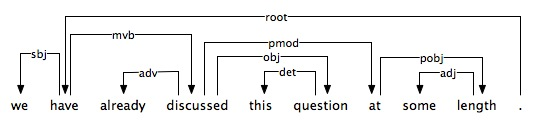
\includegraphics[width=\linewidth]{Images/dependencygrammar.jpg}
      \caption{Zin ontleed met afhankelijkheidsgrammatica\cite{GasserNotes}}
      \label{fig:dep_grammar}
  \end{figure}  

VDR's gebruiken een afhankelijkheidsgraaf om de ruimtelijke relaties tussen regio's in een foto voor te stellen. Elke relatie tussen twee objecten krijgt dan een ruimtelijke positie als label. Mogelijke relaties zijn bijvoorbeeld \texttt{op}, \texttt{boven}, \texttt{onder}, \texttt{naast}, ... Het leren van VDR's kan op basis van geannoteerde trainingsdata, automatisch met objectherkenning\cite{Elliott2015} of met nog andere informatie die in de abstracte sc\`ene zit\cite{Gilberto2015}.  

\todo[inline]{Framenet vermelden?}

\subsection{CV met neurale netwerken}
Naast deze meer traditionele manieren om informatie uit afbeeldingen af te leiden, bieden neurale netwerken een alternatieve oplossing. Voor een theoretische uitwerking van de gebruikte neurale netwerken, zie hoofdstuk \ref{hst-theorie}.

Voor de meeste taken binnen computervisie blijkt dat convolutionele neurale netwerken (CNN) beter presteren dan bovenstaande methodes.\todo{hier sta iets bij geschreven, ik denk dat het ``hoe?'' is} Deze CNN's zijn deep learning neurale netwerken met soms meer dan 15 verborgen lagen. Ze hebben minder verbindingen en parameters dan overeenkomstige feedforward neurale netwerken terwijl ze niet veel slechter presteren\cite{Krizhevsky2012a}. 
Voor verschillende CV-taken werken de huidige state-of-the-art oplossingen op basis van CNN's. Dit is onder andere het geval voor gezichtsherkenning\cite{Zhou2015}, tekenherkenning\cite{Ciresan2012} en objectherkenning\cite{Szegedy2014}.

De gebruikte CNN's binnen het automatisch beschrijven van afbeeldingen zijn getraind op ImageNet\cite{Russakovsky2014}. ImageNet is een dataset bestaande uit miljoenen afbeeldingen die gelabeld zijn binnen enkele duizenden categorie\"en. Het neuraal netwerk leert afbeeldingen correct te classificeren. Vaak gebruikte CNN modellen zijn AlexNet\cite{Krizhevsky2012a} en het recentere VGGNet\cite{Arge2015}.

Elke afbeelding dient als input voor het netwerk om zo tot een representatieve vector te komen. De meeste papers die afbeeldingen beschrijven gebruiken de gewichten van de laag voor de uiteindelijke classificatie als representatie van een afbeelding\cite{Chen2014,Karpathy2015,Mao2014a,Google}. Aandachtsgebaseerde oplossingen\cite{Jin2015,Xu2015} gebruiken ook de output van lagere convolutionele lagen als extra informatie.

Regionale CNN's vormen een variatie op CNN die een afbeelding opdeelt in verschillende interessante regio's. Hiermee is het mogelijk om voor elke regio een representatie te maken\cite{Karpathy2015,Mitchell2015}. 

\section{Representatie van zinnen}
Het is niet eenvoudig om rechtstreeks met zinnen als een geheel te werken. Daarom zijn er verschillende alternatieven onderzocht om een zin voor te stellen.
De meeste modellen vertrekken van een vectorrepresentatie voor individuele woorden. In de literatuur zijn er verschillende manieren beschreven om woordrepresentaties samen te voegen tot een representatie van een zin.

\subsection{Voorstellen van woorden}
 Het voorstellen van woorden met een vector vergemakkelijkt de verdere verwerking en kan bovendien ook semantische informatie bevatten.

 Een eerste mogelijke voorstelling is een one-hot codering waarin een vector met als grootte het aantal woorden in het vocabularium elk woord voorstelt. Deze vector is volledig nul behalve op \'e\'en rij die overeenkomt met het woord. Het is mogelijk om deze representatie verder uit breiden door vermenigvuldiging met een gewichtsmatrix. Deze matrix transformeert de one-hotvectoren naar een andere vector. Training kan zorgen voor aanpassingen aan deze gewichtsmatrix om zo ook de semantische informatie van de woorden te leren. Deze gewichtsmatrix kan willekeurig worden ge\"initialiseerd of eerst trainen op bestaande corpora\cite{Lebret2013,Mao2014a,Google}. Daarna kunnen de gekende woorden en zinnen uit de dataset de gewichten nog verfijnen.  

 Een andere mogelijkheid is om bestaande word embeddings te gebruiken zoals \texttt{word2vec}. Dat algoritme projecteert elk woord op een vooraf geleerde vector en heeft bovendien enkele mooie eigenschappen. Zo projecteert het semantisch gelijkaardige woorden op nabijgelegen posities in de vectorruimte\cite{Mikolov2013}. Deze voorgedefin\"ieerde vectoren hebben als nadeel dat niet voor elk woord uit de beschrijvingen een vector representatie beschikbaar is. Het is wel mogelijk om zelf de vectorrepresentaties te leren op basis van de gebruikte dataset zoals beschreven in de paper.

 De meeste werken in de literatuur rapporteren dat one-hotcodering in combinatie met een te leren gewichtsmatrix gelijkaardige en snellere resultaten oplevert. Daarnaast hebben sommige semantisch gelijkaardige woorden zoals kleuren gelijkaardige vectoren bij gebruik van het \texttt{word2vec} algoritme, terwijl kleuren in een afbeelding toch uitgesproken verschillend zijn. Hierdoor zal een systeem dat \texttt{word2vec} woordvectoren gebruikt, waarschijnlijk slecht presteren in het herkennen van kleuren\cite{Karpathy2015}.
 
\subsection{Voorstellen van zinnen}
 Verschillende mogelijkheden bestaan om de zinnen voor te stellen wanneer de woordvectoren gekend zijn. Een eerste mogelijkheid gebruikt een afhankelijkheidsparser en stelt de zinnen voor als een volledige afhankelijkheidsboom\cite{Socher2014}. Karpathy\cite{Karpathy2014} gebruikt ook een afhankelijkheidsparser, maar haalt hier een verzameling van triplets uit. Dergelijke triplets bestaan uit twee woorden uit de zin en hun onderlinge relatie. Figuur \ref{fig:deprelations} toont een voorbeeldzin met de bijhorende triplets. Het eerste element van de triplet is het type van de relatie.

 \begin{figure}[tb]
     \centering
     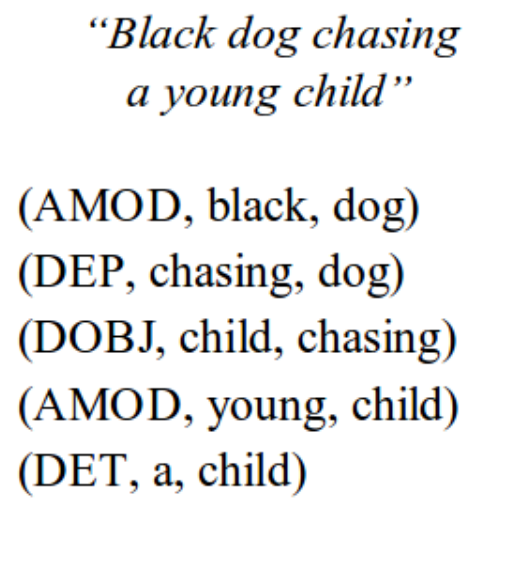
\includegraphics[width=0.35\textwidth]{Images/dep_relations}
     \caption{Zin met ontlede afhankelijkheidstriplets\cite{Karpathy2014}}
     \label{fig:deprelations}
 \end{figure}

 Een volgende optie telt de woordvectoren van een zin op\cite{Lebret2013}  Hierdoor gaat informatie uit de woordvolgorde wel verloren. Le en Mikolov\cite{Le2014a} bieden een oplossing voor het verloren gaan van woordvolgorde. Zij trainen een model om representaties te maken van stukken tekst met variabele lengte. Hun algoritme kan zowel zinnen als paragrafen en volledige teksten voorstellen.

 Een vaak gebruikt taalmodel in de meer recente NLP-literatuur is een Recurrent Neuraal Netwerk (RNN)\cite{Mikolov2010}. Dit is een neuraal netwerk dat goed overweg kan met sequenti\"ele data zoals taal. Kiros et al.\cite{Kiros2013} combineren de verborgen lagen van een RNN met extra informatie (zoals POS-tags) om tot een representatie van de zin te komen. De meer recente modellen stellen een zin voor als de sequentie van de woordvectoren in die zin. Zo kan het RNN de taal leren door elke zin woord per woord in het netwerk in te voeren.
 
\section{Van afbeeldingsrepresentaties naar beschrijvingen}
Er zijn verschillende methodes om vanuit de representaties van de afbeelding en bijbehorende referentiezinnen een model te trainen dat in staat is om ongeziene afbeeldingen om te zetten in correcte beschrijvingen. 
De meeste modellen trainen met als doel het verschil tussen de gegenereerde omschrijving en de correcte omschrijving uit de trainingsverzameling te minimaliseren.

\subsection{Dichtstbijzijnde afbeelding}
De eenvoudigste aanpak zoekt naar de meest gelijkaardige afbeelding in de trainingsverzameling en geeft \'e\'en van haar beschrijvingen terug als resultaat(Nearest Neighbour)\cite{Devlin2015a}. Een gelijkaardigheidsmetriek zoals de cosinusgelijkenis tussen de afbeeldingsrepresentaties evalueert de gelijkaardigheid van twee representaties.

Een uitbreiding op deze aanpak zoekt naar de verzameling van de meest gelijkaardige afbeeldingen in de trainingsverzameling. Vervolgens cre\"eert een model een rangorde op basis van extra visuele of tekstuele informatie. De referentiezin van de hoogst scorende afbeelding is dan het resultaat\cite{Devlin2015a,Hodosh2013,Oliva2006,Ordonez2011}. 
Deze modellen hebben als nadeel dat ze nooit resulteren in een zin die niet in de trainingsverzameling zit.

Een variatie hierop gebruikt een afbeeldingsvoorstelling met gedetecteerde objecten. Dit systeem zoekt naar de beschrijving van visueel gelijkaardige objecten in de vorm van zinsfragmenten (frases)\cite{Gupta2012,Kuznetsova2012}. Met de verzamelde fragmenten zoekt het systeem dan de meest waarschijnlijke nieuwe zin op basis van het type van de fragmenten. Deze types bestaan uit naamwoordsgroep (NP), werkwoordsgroep (VP) en voorzetselgroep (PP). De samenstelling van een nieuwe zin gebeurt dus op basis van zinsdelen die objecten gelijkaardig aan die op de foto beschrijven. De auteurs defin\"ieren meerdere beperkingen op de gegeneerde zinnen om het aantal mogelijkheden te verkleinen.

Een andere variatie op Nearest Neighbour geeft de zinnen, samen met de dichtstbijzijnde afbeelding, als input aan een tweede model. Dit model vormt deze informatie dan om tot een nieuwe zin. Zo beschouwen Mason et al.\cite{Mason2014} het genereren van beschrijvingen als een samenvattingsprobleem en gebruiken ze de beschrijvingen van gelijkaardige afbeeldingen als extra input. Analoog verkrijgen Jia et al.\cite{Fernando2015} verbeteringen op bestaande modellen door het toevoegen van extra semantische informatie zoals beschrijvingen van gelijkaardige afbeeldingen op basis van Canonical Correlation Analysis (CCA).
 
\subsection{Multimodale modellen}
Enkele werken proberen een gemeenschappelijke ruimte tussen zinnen en afbeeldingen te leren zodat het mogelijk is om de representatie van zinnen zowel als afbeeldingen op dezelfde ruimte te projecteren. Dit laat toe om afbeeldingen en zinnen rechtstreeks te vergelijken met een afstandsmaat zoals bijvoorbeeld de cosinusgelijkenis. Dit is zeer nuttig voor onder andere het opvragen van afbeeldingen met een ongeziene query en zinnen met een ongeziene afbeelding. Het leren van multimodale modellen kan onder andere met Canonical Correlation Analysis (CCA)\cite{Hodosh2013} en neurale netwerken\cite{Mao2014,Karpathy2014,Kiros2013}. 

\subsection{Sjabloongebaseerd}
Een volgende aanpak baseert zich op sjablonen om zinnen te genereren. Op basis van de gebruikte afbeeldingsvoorstelling vult een algoritme een voorgedefinieerd sjabloon in\cite{Yang2011}. Hiervoor is het dikwijls nodig om bijkomende complexe modellen te trainen\cite{Elliott2013}. Het nadeel van deze methode is dat de gegenereerde zinnen wel syntactisch correct zijn, maar dikwijls onnatuurlijk aanvoelen voor mensen. Om deze methode te verbeteren kunnen gegenereerde of vooraf gekende zinsfragmenten helpen bij het hercombineren van fragmenten\cite{Mitchell2012,Kuznetsova2012}. Daarnaast kan een algoritme een aantal gegenereerde zinnen sorteren op basis van verschillende factoren en zo de beste zin eruit halen. \todo{voorbeeld van deze factoren}

\subsection{Neurale netwerken}
De meest recente en best scorende modellen gebruiken neurale netwerken als taalmodel voor het genereren van beschrijvingen. Deze taalmodellen zijn in staat om compleet nieuwe, vlotte en natuurlijk aanvoelende zinnen te produceren. Vooral Recurrente Neurale Netwerken (RNN)\cite{Mikolov2010} winnen in de literatuur aan populariteit als taalmodel. RNN's zijn in staat om sequenti\"ele data te genereren op basis van een zekere input. LSTM's (Long Short Term Memory)\cite{SeppHochreiter1997} vormen een uitbreiding op de RNN's en onthouden informatie op lange termijn met behulp van een geheugencel.

Beide modellen verwachten een sequentie van woordrepresentaties als input, maar kunnen ook uitgebreid worden met extra informatie als invoer. Zo gebruiken meerdere werken de afbeelding als eerste invoer. Een andere toevoeging cre\"eert een multimodale ruimte tussen afbeeldingen en zinnen\cite{Kiros2014,Socher2014}. Xu et al.\cite{Xu2015} voegen een ``aandachtsvector'' toe die aangeeft waar in de afbeelding het systeem moet focussen. Het is ook mogelijk om een combinatie van verschillende technieken te gebruiken, zoals het leren van een ``sc\`enevector'' in combinatie met een aandachtsgebaseerd systeem\cite{Jin2015}. Jia et al. experimenteren met verschillende mogelijkheden om extra informatie toe te voegen, zoals CCA-projecties van afbeeldingen, of de afbeelding zelf\cite{Fernando2015}.

Een eerste verzameling van modellen met neurale netwerken volgt het codeer-decodeerprincipe uit de automatische vertaling\cite{Kiros2014}. De codeercomponent transformeert een afbeelding naar een nieuwe (multimodale) representatie. De decodeercomponent vertaalt vervolgens deze multimodale representatie naar een zin in natuurlijke taal. Door het multimodale karakter van deze modellen is het opvragen van afbeeldingen en zinnen ook mogelijk. Dit opvragen gebeurt door middel van projectie van een nieuwe afbeelding of zin in de multimodale ruimte. Een vergelijking van deze projectie met de zinnen of afbeeldingen uit de trainingsverzameling leidt tot een rangschikking van de trainingsvoorbeelden. Er bestaan zowel codeer-decodeer modellen met LSTM's\cite{Kiros2014} als met RNN's\cite{Karpathy2014,Mao2014a}.

Een tweede categorie gebruikt zowel de afbeeldingsrepresentatie als de sequentie van 
woordrepresentaties als input bij het trainen van het netwerk. Op basis van een trainingsafbeelding probeert het netwerk het eerste woord uit de zin te voorspellen. Deze voorspelling dient dan, al dan niet samen met de afbeelding, als input voor de voorspelling van het volgende woord. Terugpropagatie van de fout op de gegenereerde woorden doorheen het netwerk zorgt voor de juiste wijzigingen aan de gewichten. Op deze manier leert het netwerk om op basis van een ongeziene afbeelding de juiste sequentie van woorden te genereren. Ook hier bestaan er modellen met LSTM's\cite{Donahue2015,Google} en RNN's\cite{Karpathy2015}. \todo{meer papers toevoegen}

Het trainen van deze netwerken gebeurt doorgaans met terugpropagatie doorheen het netwerk. Het is mogelijk om de fouten ook verder door te propageren naar de gewichtsvectoren van de woordrepresentaties of naar de gewichten van een CNN. Die methode optimaliseert op die manier alle gewichten op de dataset, maar kan computationeel kostelijk zijn.

Alle neurale netwerken gebruikt in deze thesis hebben een ``softmax'' als laatste laag. Deze laag zorgt ervoor dat het netwerk een kansverdeling genereert voor het volgende woord. Het meest waarschijnlijke woord heeft dan de hoogste kans.
Het selecteren van het woord voor de generatie kan gebeuren door het samplen van deze verdeling, of door het gebruik van een zoekalgoritme zoals beam search, om zo de meest waarschijnlijke beschrijving te benaderen. Een specifiek stopwoord kenmerkt zowel het begin als het einde van de zin.

\subsection{Statistische taalmodellen}
Naast de neurale netwerken behoren ook de statistische taalmodellen tot de beter scorende modellen. Deze modellen proberen op basis van entropie een taal zo goed mogelijk te beschrijven. Entropie is een maat voor informatie en heeft verschillende doeleinden binnen het domein van NLP. 

Concreet stelt de entropie $H$ de hoeveelheid informatie voor die in een willekeurige variabele $X$ zit. $X$ is typisch de voorspelde variabele. Bij het afbeeldingsbeschrijvingsprobleem zijn dit typisch woorden of zinnen. Het domein van deze variabele is $\chi$. De entropie van $X$ is te berekenen met formule \eqref{entropy}, waarbij $p(x)$ de kans voorstelt dat $X$ waarde $x$ heeft\cite{Jurafsky:2009:SLP:1214993}. 

\begin{equation}
     H(X) = -\sum_{x \in \chi}p(x)\log_2p(x)
     \label{entropy}
 \end{equation} 

Entropie-gebaseerde modellen modelleren de kennis die zeker is en ze beschouwen onzekerheden als uniform. Als een woord vijf mogelijke vertalingen heeft, waar het systeem verder niets over weet, heeft elke vertaling een kans van $\frac{1}{5}$. Als het systeem uit observatie weet dat in 50 \% van de gevallen een van de eerste 2 vertalingen is, hebben deze twee vertalingen een waarschijnlijkheid van $\frac{1}{4}$. De andere drie vertalingen, waarover het systeem onzeker is, hebben een waarschijnlijkheid van $\frac{1}{6}$, wat neerkomt op een uniforme kansverdeling binnen de beperkingen die uit de observaties voortkomen. In andere modellen kunnen deze beperkingen voortkomen uit sjablonen, het al dan niet observeren van bepaalde woordsequenties, \ldots \cite{Berger1996}

Zo leren Mitchell et al.\cite{Mitchell2015} om een lijst met waarschijnlijke woorden uit de afbeeldingsrepresentatie te extraheren en combineren ze deze met een uitgebreid taalmodel. Dit taalmodel leert de verschillende kansen op basis van de beschrijvingen in de trainingsdata. Tijdens het leerproces probeert het algoritme de entropie te maximaliseren. In een volgende stap van hun systeem zoeken ze de zinnen die het meest waarschijnlijk zijn, gegeven de woorden die herkend zijn in de afbeelding. Vervolgens sorteren ze de gegeneerde zinnen op basis van een aantal additionele kenmerken. Dit model is net als de modellen met neurale netwerken in staat om nieuwe en vlotte zinnen te vormen. De prestatie is gelijkaardig aan die van de neurale netwerken.

Lebret\cite{Lebret2015} toont bovendien aan dat een nog eenvoudiger taalmodel toch relatief goede resultaten kan bekomen. Dit model extraheert alle zinsfragmenten (frases) uit de trainingsdata en leert daarmee een eenvoudig 3-gram taalmodel. Voor ongeziene afbeeldingen bepaalt het model de best overeenkomende zinsfragmenten en probeert hiermee zinnen te maken. In tegenstelling tot alle voorgaande modellen gebeurt training van deze multimodale transformatie met negatieve sampling. Hierbij leert het model een juiste referentiezin te onderscheiden in een lijst die ook willekeurig gekozen zinnen bevat. Ook hier gebeurt er aan het einde nog een hersortering van de gegenereerde zinnen op basis van de overeenstemming met de afbeelding.

\subsection{Aandachtsgebaseerde modellen}
State-of-the-art modellen uit het automatisch vertalen gebruiken mechanismes die aandachtsgebaseerd zijn. Concreet betekent dit dat het decodeeralgoritme zelf beslist welke stukken uit de zin meer aandacht vereisen.
In de setting van het beschrijven van afbeeldingen komt dit neer op een mechanisme dat aangeeft welke regio's in de afbeelding belangrijk zijn. In de decoder zorgt dit aandachtsmechanisme voor een extra contextvector als input voor een neuraal netwerk. 

Deze aandachtsvector kan zowel ``hard'' als ``zacht'' zijn. ``Harde'' aandacht is een stochastisch principe dat de aandachtslocatie beschouwt als een latente variabele. Tijdens elke stap samplet\todo{Nederlands woord?} het algoritme \'e\'en locatie om de aandacht op te vestigen tijdens het genereren van het volgende woord. ``Zachte'' aandachtsmethodes werken deterministisch, waardoor er geen nood is om elke stap een sample-operatie uit te voeren. Een differentieerbare functie bepaalt de aandachtslocatie tijdens elke stap van het trainingsproces. Door de differentieerbaarheid is het netwerk dat de aandachtsvector berekent eenvoudig te trainen met behulp van terugpropagatie.

Aandachtsmodellen geven bovendien een mooie visuele voorstelling van waar het model bepaalde woorden ``ziet'' (figuur \ref{fig:attention-example}). Binnen het automatisch beschrijven van afbeeldingen bereiken deze aandachtsgebaseerde modellen voorlopig de beste resultaten\cite{Jin2015,Xu2015}.

\begin{figure}[tb]
	\centering
	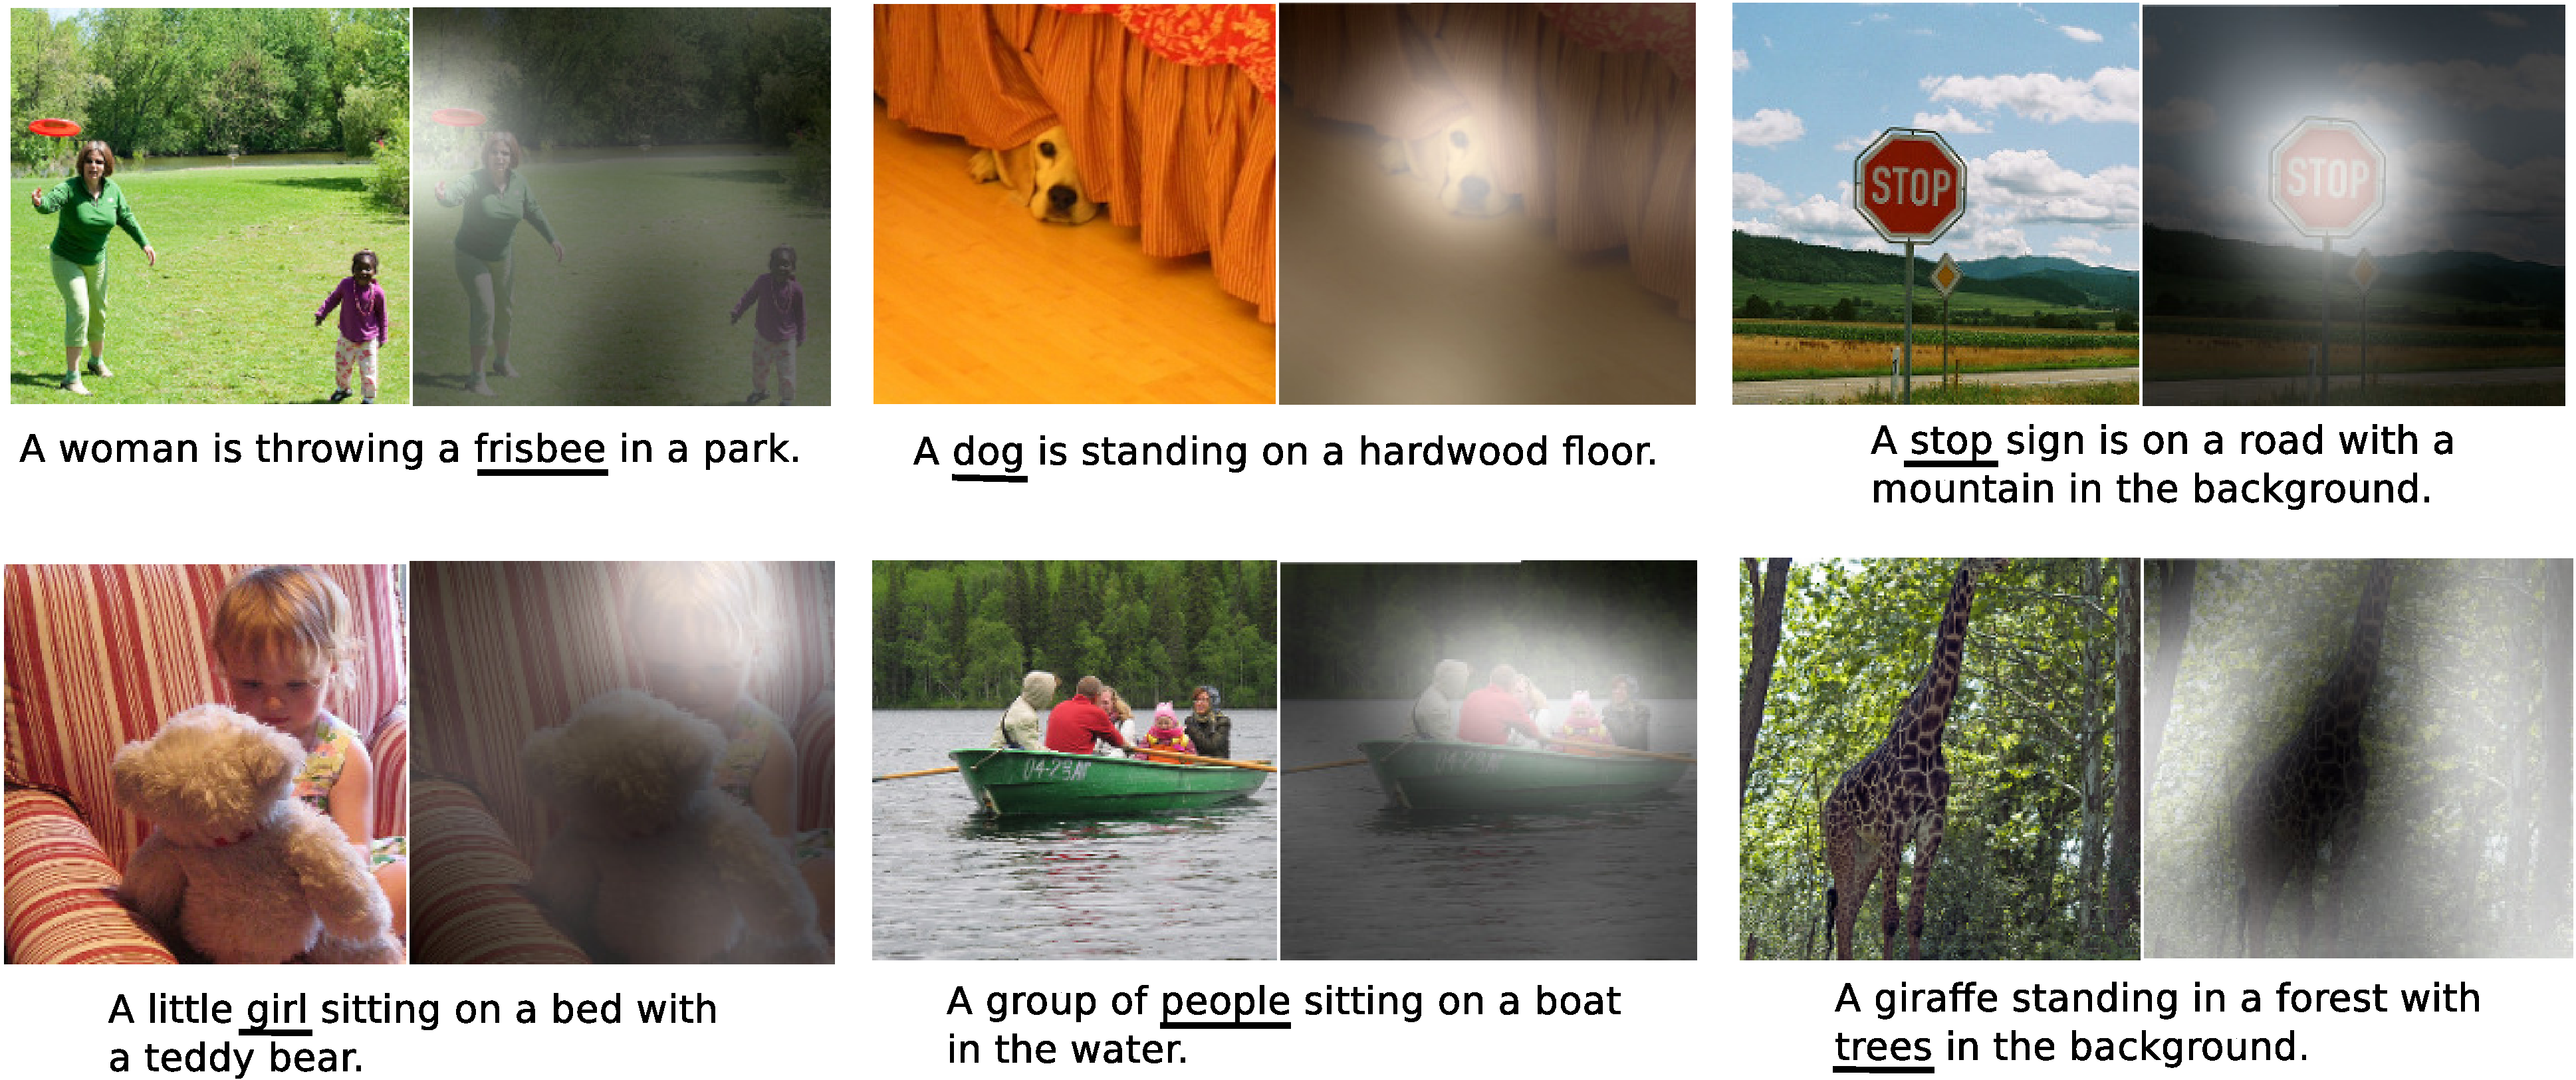
\includegraphics[width=\linewidth]{Images/good_Xu.pdf}
	\caption[Voorbeelden van aandacht op correcte regio.]{Voorbeelden van aandacht op correcte regio. (Wit in de afbeelding is de gefocuste regio, onderlijnde tekst is het overeenkomstige woord)\cite{Xu2015}}
	\label{fig:attention-example}
\end{figure}


\section{Besluit}
%%% Local Variables: 
%%% mode: latex
%%% TeX-master: "masterproef"
%%% End: 
\chapter{Een volgend hoofdstuk}
\label{hoofdstuk:2}
Een hoofdstuk behandelt een samenhangend geheel dat min of meer op zichzelf
staat. Het is dan ook logisch dat het begint met een inleiding, namelijk
het gedeelte van de tekst dat je nu aan het lezen bent.

\section{Eerste onderwerp in dit hoofdstuk}
De inleidende informatie van dit onderwerp.

\subsection{Een item}
Een tekst staat nooit alleen. Dit wil zeggen dat er zeker ook referenties
nodig zijn. Dit kan zowel naar on-line documenten\cite{wiki} als naar
boeken\cite{pratchett06:_good_omens}.

\section{Figuren}
Figuren worden gebruikt om illustraties toe te voegen. Dit is dan ook de
manier om beeldmateriaal toe te voegen zoals getoond wordt in
figuur~\ref{fig:logo}.

\begin{figure}
  \centering
  \includegraphics{logokul}
  \caption{Het KU~Leuven logo.}
  \label{fig:logo}
\end{figure}

\section{Tabellen}
Tabellen kunnen gebruikt worden om informatie op een overzichtelijke te
groeperen. Een tabel is echter geen rekenblad! Vergelijk maar eens
tabel~\ref{tab:verkeerd} en tabel~\ref{tab:juist}. Welke tabel vind jij het
duidelijkst?

\begin{table}
  \centering
  \begin{tabular}{||l|lr||} \hline
    gnats     & gram      & \$13.65 \\ \cline{2-3}
              & each      & .01 \\ \hline
    gnu       & stuffed   & 92.50 \\ \cline{1-1} \cline{3-3}
    emu       &           & 33.33 \\ \hline
    armadillo & frozen    & 8.99 \\ \hline
  \end{tabular}
  \caption{Een tabel zoals het niet moet.}
  \label{tab:verkeerd}
\end{table}

\begin{table}
  \centering
  \begin{tabular}{@{}llr@{}} \toprule
    \multicolumn{2}{c}{Item} \\ \cmidrule(r){1-2}
    Animal    & Description & Price (\$)\\ \midrule
    Gnat      & per gram    & 13.65 \\
              & each        & 0.01 \\
    Gnu       & stuffed     & 92.50 \\
    Emu       & stuffed     & 33.33 \\
    Armadillo & frozen      & 8.99 \\ \bottomrule
  \end{tabular}
  \caption{Een tabel zoals het beter is.}
  \label{tab:juist}
\end{table}

\section{Lorem ipsum}
Tenslotte gaan we hier nog wat tekst voorzien zodat er minstens een
bijkomende bladzijde aangemaakt wordt. Dat geeft de gelegenheid om eens te
zien hoe de koptekst en de voettekst zich gedragen.

\subsection{Lorem ipsum dolor sit amet, consectetur adipiscing elit}
Sed nec tortor id felis tristique sodales. Nulla nec massa eu dui fermentum
tincidunt. Integer ullamcorper ante eget eros posuere faucibus. Nam id
ligula ut augue pulvinar vulputate id at purus. Aenean condimentum tortor
eu mi placerat eget eleifend massa mollis. Nam est mi, sagittis quis
euismod eget, sagittis in nibh. Proin elit turpis, aliquam et imperdiet
sed, volutpat eu turpis.

Pellentesque vel enim tellus, vitae egestas turpis. Praesent malesuada elit
non nisi sollicitudin non blandit lacus tincidunt. Morbi blandit urna at
lectus ornare laoreet. Suspendisse turpis diam, lobortis dictum luctus
quis, commodo at lorem. Integer lacinia convallis ultricies. Sed quis augue
neque, eu malesuada arcu. Nullam vehicula, purus vitae sagittis pulvinar,
erat eros semper massa, eu egestas nibh erat quis magna. Cras pellentesque,
nisl eu dapibus volutpat, urna augue ornare quam, quis egestas lectus nulla
a lectus.

Vivamus dictum libero in massa cursus sed vulputate eros imperdiet. Donec
lacinia, libero ac lobortis egestas, nibh dui ornare arcu, luctus porttitor
velit massa sit amet quam. Maecenas scelerisque laoreet diam, vitae congue
quam adipiscing vitae. Aliquam cursus nisl a leo convallis eleifend
fermentum massa porta. Nunc libero quam, dapibus dapibus molestie sit amet,
faucibus vel nunc.

\subsection{Praesent auctor venenatis posuere}
Sed tellus augue, molestie in pulvinar lacinia, dapibus non ipsum. Fusce
vitae mi vitae enim ullamcorper hendrerit eu malesuada est. Proin iaculis
ante sed nibh tincidunt vel interdum libero posuere. Vivamus accumsan metus
quis felis congue suscipit dapibus enim mattis. Fusce mattis tortor eget
ipsum interdum sagittis auctor id metus.

Integer diam lacus, pharetra sit amet tempor et, tristique non lorem.
Aenean auctor, nisi eu interdum fermentum, lectus massa adipiscing elit,
sed facilisis orci odio a lectus. Proin mi nibh, tempus quis porta a,
viverra quis enim. In sollicitudin egestas libero, quis viverra velit
molestie eget. Nulla rhoncus, dolor a mollis vestibulum, lacus elit semper
nisi, nec sollicitudin sem urna eu magna. Nunc sed est urna, euismod congue
mi.

\subsection{Cras vulputate ultricies venenatis}
Vivamus eros urna, sodales accumsan semper vel, lobortis sit amet mauris.
Etiam condimentum eleifend lorem, ullamcorper ornare lectus aliquet vitae.
Praesent massa enim, interdum sit amet semper et, venenatis ut elit.
Quisque faucibus, quam ac lacinia imperdiet, nulla neque elementum purus,
tempus rutrum justo massa porta sapien. Vestibulum ante ipsum primis in
faucibus orci luctus et ultrices posuere cubilia Curae; Sed ultrices
interdum mi, et rhoncus sapien rutrum sed.

Duis elit orci, molestie quis sollicitudin sed, convallis non ante.
Maecenas tincidunt condimentum justo, et ultricies leo tristique vitae.
Vestibulum quis quam non lectus dapibus eleifend a vitae nibh. Nam nibh
justo, pharetra quis iaculis consequat, elementum quis justo. Etiam mollis
lacinia lacus, nec sollicitudin urna lobortis ac. Nulla facilisi.

Proin placerat risus eleifend erat ultricies placerat. Etiam rutrum magna
nec turpis euismod consectetur. Phasellus tortor odio, lacinia imperdiet
condimentum sed, faucibus commodo erat. Phasellus sed felis id ante
placerat ultrices. Aenean tempor justo in tortor volutpat eu auctor dolor
mollis. Aenean sit amet risus urna. Morbi viverra vehicula cursus.

\subsection{Donec nibh ante, consectetur et posuere id, tempus nec arcu}
Curabitur a tellus aliquet ipsum pellentesque scelerisque. Etiam congue,
risus et volutpat rutrum, est purus dapibus leo, non cursus metus felis
eget ligula. Vivamus facilisis tristique turpis, ut pretium lectus luctus
eleifend. Fusce magna sapien, ullamcorper vitae fringilla id, euismod quis
ante.

Phasellus volutpat, nunc et pharetra semper, sem justo adipiscing mauris,
id blandit magna quam et orci. Vestibulum a erat purus, ut molestie ante.
Vestibulum ante ipsum primis in faucibus orci luctus et ultrices posuere
cubilia Curae; Proin turpis diam, consequat ut ullamcorper ut, consequat eu
orci. Sed metus risus, fringilla nec interdum vel, interdum eu nunc.
Suspendisse vel sapien orci.

\subsection{Morbi et mauris tempus purus ornare vehicula}
Mauris sit amet diam quam, eget luctus purus. Sed faucibus, risus semper
eleifend iaculis, mi turpis bibendum nisl, quis cursus nibh nisl sit amet
ipsum. Vestibulum tempor urna vitae mi auctor malesuada eget non ligula.
Nullam convallis, diam vel ultrices auctor, eros eros egestas elit, sed
accumsan arcu tortor eget leo. Vestibulum orci purus, porttitor in pharetra
eget, tincidunt eget nisl. Nullam sit amet nulla dui, facilisis vestibulum
dui.

Donec faucibus facilisis mauris ac cursus. Duis rhoncus quam sed nisi
laoreet eu scelerisque massa tincidunt. Vivamus sit amet libero nec arcu
imperdiet tempor quis non libero. Sed consequat dignissim justo. Phasellus
ullamcorper, velit quis posuere vulputate, felis erat tincidunt mauris, at
vestibulum justo lectus et turpis. Maecenas lacinia convallis euismod.
Quisque egestas fermentum sapien eu dictum. Sed nec lacus in purus dictum
consequat quis vel nisl. Fusce non urna sem. Curabitur eu diam vitae elit
accumsan blandit. Nullam fermentum nunc et leo dictum laoreet. Donec semper
varius velit vel fringilla. Vivamus eu orci nunc.

\section{Besluit van dit hoofdstuk}
Als je in dit hoofdstuk tot belangrijke resultaten of besluiten gekomen
bent, dan is het ook logisch om het hoofdstuk af te ronden met een
overzicht ervan. Voor hoofdstukken zoals de inleiding en het
literatuuroverzicht is dit niet strikt nodig.

%%% Local Variables: 
%%% mode: latex
%%% TeX-master: "masterproef"
%%% End: 

% ... en zo verder tot
\chapter{Het laatste hoofdstuk}
\label{hoofdstuk:n}
Een hoofdstuk behandelt een samenhangend geheel dat min of meer op zichzelf
staat. Het is dan ook logisch dat het begint met een inleiding, namelijk
het gedeelte van de tekst dat je nu aan het lezen bent.

\section{Eerste onderwerp in dit hoofdstuk}
De inleidende informatie van dit onderwerp.

\subsection{Een item}
De bijbehorende tekst. Denk eraan om de paragrafen lang genoeg te maken en
de zinnen niet te lang.

Een paragraaf omvat een gedachtengang en bevat dus steeds een paar zinnen.
Een paragraaf die maar \'e\'en lijn lang is, is dus uit den boze.

\section{Tweede onderwerp in dit hoofdstuk}
Er zijn in een hoofdstuk verschillende onderwerpen. We zullen nu
veronderstellen dat dit het laatste onderwerp is.

\section{Besluit van dit hoofdstuk}
Als je in dit hoofdstuk tot belangrijke resultaten of besluiten gekomen
bent, dan is het ook logisch om het hoofdstuk af te ronden met een
overzicht ervan. Voor hoofdstukken zoals de inleiding en het
literatuuroverzicht is dit niet strikt nodig.

%%% Local Variables: 
%%% mode: latex
%%% TeX-master: "masterproef"
%%% End: 

\chapter{Besluit}
\label{besluit}
Deze masterproef probeert twee bestaande systemen voor afbeeldingsbeschrijving te verbeteren. Deze systemen gebruiken een convolutioneel neuraal netwerk om een afbeelding om te zetten tot een vectorvoorstelling. Deze voorstelling is de input van een taalmodel op basis van een recurrent neuraal netwerk. Samen met een beam-search-algoritme is dit taalmodel in staat om beschrijvingen te genereren.

De verbeteringen ten opzichte van de bestaande systemen gebeuren op drie manieren. Ten eerste is er het afleiden van extra informatie uit een afbeelding, hetzij door het extraheren van onderwerpen, hetzij door een multimodale projectie. Beide gebruikte methodes zijn variabel in het aantal gebruikte dimensies. Deze masterproef bestudeert dan ook de invloed van de dimensionaliteit van de extra informatie. 
De recente dataset Flickr30kEntities vormt een derde bron van informatie, maar blijkt in deze opstelling te groot om mee te werken.
Een tweede aangebrachte verbetering is het normaliseren van de zinnen tijdens het generatieproces. Dit kan leiden tot zinnen die meer informatie bevatten of tot een betere verdeling van de zinslengtes. Tenslotte bestudeert deze masterproef de mogelijke invloed van een aantal parameters van het generatieproces.

De automatische evaluatiemethodes BLEU en Meteor uit de machinevertaling maken een objectieve vergelijking van de verschillende systemen mogelijk. Daarnaast bieden statistieken over woordgebruik, zinslengte en uniciteit van de gegenereerde zinnen verdere inzichten.

Deze thesis experimenteert ook met de robuustheid van de twee manieren om semantische informatie toe te voegen. Een aantal experimenten bepaalt de invloed van ruis op deze informatie.

Dit hoofdstuk biedt eerst een overzicht van de belangrijkste resultaten en verbeteringen, en hoe die een antwoord geven op de geponeerde onderzoeksvragen. Daarna volgt een overzicht van de mogelijke uitbreidingen.
\section{Resultaten}
Deze sectie biedt een overzicht van de behaalde resultaten. De volgende onderdelen focussen telkens op het beantwoorden van \'e\'en of meerdere onderzoeksvragen, zoals gesteld in sectie~\ref{sec:vragen}.
\subsection{Toevoegen van semantische informatie}
\emph{Welke vormen van semantische informatie kunnen op een haalbare manier verbetering bieden voor bestaande systemen?}

Experimenten met het gebruik van de Flickr30k Entities wijzen uit dat het niet haalbaar is om deze dataset om te zetten naar bruikbare informatie. Het gebruik van zowel afgeleide onderwerpverdelingen en multimodale projecties is computationeel minder complex en biedt mogelijkheden tot integratie.

\emph{Hoe kan semantische informatie worden toegevoegd aan de twee bestudeerde systemen?}

Het toevoegen van een vector met semantische informatie aan het bestudeerde RNN gebeurt door de informatie bij de input op te tellen. Bij het uitbreiden van het LSTM-netwerk volgen we de aanpak van Jia et al.~\cite{Fernando2015}. De vector dient dan als gids voor het netwerk.

\emph{Hoe presteren verschillende types van semantische informatie ten opzichte van elkaar?}

Het gebruik van extra semantische informatie leidt tot verbeteringen in de kwaliteit van de gegenereerde zinnen. 
Bij RNN zorgt het gebruik van de onderwerpen afgeleid uit de afbeeldingen voor een hogere score ten opzichte van het referentiemodel. 
De veronderstelling dat de onderwerpen de gegenereerde zinnen beter doet aansluiten bij de afbeelding is dus correct.
Bij LSTM geven zowel de afgeleide onderwerpen als de multimodale projectie een hogere score dan het referentiemodel. 
De scores van beide technieken om extra informatie toe te voegen liggen bij LSTM zeer dicht bij elkaar, maar het gebruik van onderwerpen scoort lichtjes beter op de metrieken die het dichtst aanleunen bij menselijke evaluatie.

\subsection{Normalisatie}
\emph{Hoe kunnen we langere, minder algemene zinnen genereren?}

Om de lengte van de gegenereerde zinnen beter te doen aansluiten bij die van de trainingsverzameling implementeert deze masterproef een Gaussfunctie. Hierdoor krijgen zinnen die te veel afwijken van de lengteverdeling uit de trainingsset een lagere score. 
Deze methode heeft een zeer grote invloed op de gegenereerde zinnen. De gemiddelde lengte stijgt bij RNN van 7 naar 10 en bij LSTM van 8 naar 10. Voor de belangrijkste evaluatiemethodes verbetert deze normalisatie ook de kwaliteit.

Een tweede vorm van normalisatie probeert de gegenereerde zinnen informatiever te maken. Alle woorden uit de woordenschat krijgen een score op basis van de frequentie van voorkomen in de trainingsverzameling. Woorden die minder voorkomen zijn specifieker en krijgen een hogere score. Op basis van deze scores krijgen de woorden in de gegenereerde zinnen een aangepast gewicht. Deze normalisatie leidt effectief tot zinnen die een groter aantal veelzeggende woorden bevatten. Dikwijls leidt dit ook tot een zin van hogere kwaliteit, maar in een aantal gevallen voegt het systeem schijnbaar willekeurig een aantal woorden met een hoge score toe die weinig met de afbeelding te maken hebben. De evaluatiemetrieken oordelen ook dat de zinnen met deze normalisatie in zijn geheel slechter presteren, maar voor een mens zijn een groot aantal van de zinnen wel van betere kwaliteit.

\subsection{Invloed van parameters}
\emph{Wat is de invloed van het aanpassen van systeemspecifieke parameters?}

Verschillende parameters van het systeem hebben een invloed op de resultaten. Ten eerste is er de grootte van de beam-search bij het zoeken van de beste beschrijvingen. Naarmate de grootte stijgt zijn de scores beter, tot aan een plafond. Afhankelijk van het gebruikte systeem ligt de optimale grootte tussen 25 en 75. Ook de dimensionaliteit van de vector met extra semantische informatie heeft een invloed. Bij het gebruik van onderwerpverdelingen is de invloed variabel. Bij langere zinnen, bijvoorbeeld door Gauss-normalisatie, is het beter om een groter aantal onderwerpen te kiezen. Voor kortere zinnen verzwakt dit effect. Bij multimodale projectie is dit fenomeen niet zichtbaar. De modellen die gebruik maken van 256 dimensies scoren wel beter dan die met 128 en 512 dimensies. Bij 128 dimensies is de informatie wellicht te beperkt. Bij 512 daarentegen komen veel onbelangrijke elementen in de vector die doorwegen in het uiteindelijke resultaat.

\subsection{Robuustheid van semantische informatie}
\emph{Welke invloed ondervinden de beschouwde types semantische informatie van trainingsdata die ruis bevat?}

Beide methodes om semantische informatie toe te voegen aan de bestudeerde systemen ondervinden nadeel van ruis op de trainingsdata. Deze ruis bestaat erin elk woord met een kans van 10\% te vervangen door een willekeurig ander woord. De absolute en relatieve achteruitgang is kleiner bij het gebruik van een multimodale projectie. Dit komt vermoedelijk omdat het netwerk dan slechter in staat is om het verband te leren tussen de trainingszinnen en de vector met extra informatie.

\subsection{Beste resultaten}
Wij beschouwen LSTM met een zelf ge\"introduceerde gidsvector op basis van onderwerpverdelingen met 120 onderwerpen als het best presterende systeem. Gaussnormalisatie en een beam-search met grootte 50 leiden tot de hoogste scores.  De vergelijking van de systemen is gemaakt op basis van de hogere BLEU-scores en Meteor, aangezien die het meest correleren met menselijke beoordelingen. Ons systeem presteert zeer gelijkaardig in vergelijking met de meest recente literatuur. Het moet voornamelijk onderdoen voor aandachtsgebaseerde systemen. 

Het gebruik van ons RNN met onderwerpverdelingen van lengte 120 en Gaussnormalisatie presteert iets slechter, maar is veel sneller te trainen. Wanneer de trainingstijd beperkt is of bij het gebruik van een hele grote dataset kan RNN alsnog een waardig alternatief vormen.

\section{Toekomstig werk}
Deze sectie geeft een korte samenvatting van een aantal punten waar in de toekomst verbeteringen mogelijk zijn.

Het trainen van een model met een bepaalde keuze van parameters duurt steeds ongeveer een week op de gebruikte hardware. Om die reden zijn veel van de instelbare parameters in de implementatie nooit gewijzigd. Het loont dus zeker de moeite om te onderzoeken of door wijziging hiervan de resultaten verbeteren.

De huidige modellen struikelen nog steeds over een aantal problemen. Zo is de kwaliteit van de afbeeldingsvoorstelling zeker belangrijk. Betere convolutionele netwerken kunnen hiervoor zorgen. Daarnaast heeft het huidige systeem last met het toewijzen van kleur aan het juiste object. Ook aantallen vormen dikwijls een probleem. Oplossingen hiervoor zijn dus nog nodig.

Bij het onderzoek naar het ideale aantal onderwerpen van LDA, was 120 het best scorende model met Gauss-normalisatie. Het kan interessant zijn om te kijken of een nog groter aantal deze resultaten nog verhoogt en waar net de bovengrens op dit aantal ligt.

Idf-normalisatie zorgt voor creatievere en meer unieke zinnen. Helaas genereert het ook vaak compleet foute beschrijvingen. 
Verder onderzoek naar variaties op deze normalisatie lijkt nuttig. Wanneer deze fouten zouden verdwijnen, lijken de zinnen immers menselijker.

Zoals beschreven in het literatuuroverzicht en de resultaten scoren de modellen die gebruik maken van aandachtsmechanismes het hoogste. Het gebruik van aandachtsvectoren is echter te complex voor deze masterproef. Het is zeker interessant om te experimenteren met het toevoegen van aandachtsinformatie aan de systemen voorgesteld in deze masterproef. De literatuur leert ons dat verbetering zeker nog mogelijk is. 

Een ander mogelijk vervolg op deze masterproef gaat dieper in op de robuustheid van de verschillende systemen om semantische informatie toe te voegen aan de generatiesystemen.
De aanpak in de experimenten is vrij rudimentair, dus het zou zeker lonen om te onderzoeken wat de invloed is van verschillende gradaties van aanpassingen in de trainingsset, alsook verschillende types van ruis.

Een laatste mogelijke verderzetting van dit werk focust op de toepassing van de automatische afbeeldingsbeschrijving. 
Zo is verder onderzoek nodig naar de integratie van dit en soortgelijke systemen in browsers en applicaties voor blinden en slechtzienden. Facebook~\cite{facebook} gebruikt ondertussen al automatische afbeeldingsbeschrijving in hun toepassingen voor slechtzienden. Hierbij beschrijft een stem wat er zich op een geselecteerde afbeelding bevindt. Een algemene browser die elke foto automatisch omzet in een beschrijving en deze bijvoorbeeld voorleest, heeft dus zeker zijn praktisch nut.

%%% Local Variables: 
%%% mode: latex
%%% TeX-master: "masterproef"
%%% End: 


% Indien er bijlagen zijn:
\appendixpage*          % indien gewenst
\appendix
\chapter{De eerste bijlage}
\label{app:A}
In de bijlagen vindt men de data
% ... en zo verder tot
\chapter{De laatste bijlage}
\label{app:n}
In de bijlagen vindt men de data terug die nuttig kunnen zijn voor de
lezer, maar die niet essentieel zijn om het betoog in de normale tekst te
kunnen volgen. Voorbeelden hiervan zijn bronbestanden,
configuratie-informatie, langdradige wiskundige afleidingen, enz.

\section{Lorem 20-24}
\lipsum[20-24]

\section{Lorem 25-27}
\lipsum[25-27]

%%% Local Variables: 
%%% mode: latex
%%% TeX-master: "masterproef"
%%% End: 


\backmatter
% Na de bijlagen plaatst men nog de bibliografie.
% Je kan de  standaard "abbrv" bibliografiestijl vervangen door een andere.
\bibliographystyle{abbrv}
\bibliography{referenties}

\end{document}

%%% Local Variables: 
%%% mode: latex
%%% TeX-master: t
%%% End: 
